%!TEX root = ../thesis.tex
\chapter{Побудова моделей та оцінка методів}
\label{chap:practice}

У цьому розділі описано налаштування гіперпараметрів моделей MLP та $(1+\lambda)$-EA with GP encoding, а також порівняння їхньої ефективності на основі метрик accuracy, precision, recall та f1-score. Моделі перевірялися на різних наборах даних для задач бінарної та багатокласової класифікації.

\section{Детальний опис моделей та підбір гіперпараметрів моделей}

Як вже було зазначено в даній роботі ми сфокусувалися на тестуванні моделей MLP with gradient descent, MLP with single-point mutation та $(1+\lambda)$-EA with GP encodings. Принцип тренування MLP with gradient descent ми описали в розділі \ref{sec:training_process}, тому в цьому розділі ми опишемо детально процес навчання моделей MLP with single-point mutation та $(1+\lambda)$-EA with GP encoding.

MLP with single-point mutation використовує оптимізаційний алгоритм, який працює наступним чином: на кожній епосі випадковим чином обирається значення однієї ваги з усієї нейронної мережі -- $w_{ij}$ та до нього додається значення випадкової величини, яка має нормальний розподіл з нульовим математичним сподіванням та певним значенням дисперсії. Після цього розраховується функція втрат з оновленими вагами, якщо її значення стало менше, ніж було з початковими вагами на поточній епосі, то ваги зберігаються і процес переходить на наступну епоху, якщо функція втрат збільшилася, то повертаються ваги, які були до додавання значення випадкової величини і відбувається перехід на наступну епоху. Цей процес повторюється задану кількість епох. У вигляді псевдокоду це можна записати як:

\begin{algorithm}
	\caption{MLP with single-point mutation}
	\begin{algorithmic}[1]
		\STATE Вибір випадкового вагового коефіцієнта: $w_{ij}$
		\STATE $\epsilon \sim \mathcal{N}(0, \sigma^2)$
		\STATE $w_{ij} \gets w_{ij} + \epsilon$
		\IF{$loss_{new} < loss_{old}$}
		\STATE $w_{ij} \gets w_{ij}$
		\ELSE
		\STATE $w_{ij} \gets w_{ij} - \epsilon$
		\ENDIF
	\end{algorithmic}
\end{algorithm}

\vspace{1cm}

Метод $(1+\lambda)$-EA with GP encoding описується наступним чином. Першим кроком ініціалізується індивід, в нашому випадку індивідом є дерево у якого в якості внутрішніх вузлів -- функції, які мають арність 2, а в якості листків -- ознаки датасету або константи з набору: $1, 0, -1, e, \pi$. Для цього індивіду розраховується фітнес-функція. Після того, як була розрахована фітнес-функція для створеного індивіду, він мутує $\lambda$ разів, таким чином ми отримуємо $\lambda$ нових індивідів. Мутація в даному випадку відбувається наступним чином: випадково обирається один вузол з усього індивіду і його значення замінюється на якесь інше випадкове, валідне значення (у випадку внутрішніх вузлів -- значення замінюється на якусь іншу функцію, а у випадку листків на якусь іншу ознаку, або константу).  Після цього ми розраховуємо фітнес-функції для усіх новостворених індивідів і обираємо індивід, який має найменше значення фітнес-функцї. Цей індивід далі виступає в ролі батька на наступних ітераціях. У вигляді псевдокоду це можна представити як:

\begin{algorithm}
	\caption{$(1+\lambda)$-EA with GP encoding}
	\begin{algorithmic}[1]
		\STATE $x_0 \gets \text{випадковий початковий генотип}$
		\WHILE{не виконано}
		\FOR{$i \in 1, \ldots, \lambda$}
		\STATE $x_i \gets \text{мутація}(x_0)$
		\ENDFOR
		\FOR{$i \in 1, \ldots, \lambda$}
		\IF{$f(x_i) < f(x_0)$}
		\STATE $x_0 \gets x_i$
		\ENDIF
		\ENDFOR
		\ENDWHILE
	\end{algorithmic}
\end{algorithm}

Тепер після того, як ми описали, як в нашому випадку працюють алгоритми, перейдемо до процесу підбору оптимальних гіперпараметрів. Процес вибору гіперпараметрів є важливим кроком в тренуванні моделей, оскільки від них значно залежить швидкість конвергенції та якість моделей. Тому в цій частині ми опишемо, процес за яким відбувається підбір гіперпараметрів для різних задач та моделей, а також які саме гіперпараметри виявилися оптимальними і які ми використовуємо.

Почнемо розгляд з задач класифікації та моделі MLP with gradient descent. Для підбору гіперпараметрів для цієї моделі ми використовували бібліотеку optuna, яка дозволяє проводити байєсівську оптимізацію~\cite{ct37}. Для цього ми задали простір гіперпараметрів по якому проводився пошук оптимальних з них за 1000 ітерацій. Оптимальні гіперпараметри для кожної задачі можна подивитися у таблиці \ref{tab_hyperparameters_for_mlp_with_gd}.

\begin{table}[ht]
	\centering
	\begin{adjustbox}{max width=\textwidth}
		\begin{tabular}{|c|p{3cm}|p{3cm}|p{3cm}|p{3cm}|}
			\hline \multirow{2}{*}{Гіперпараметри} & \multicolumn{4}{c|}{Задачі} \\
			\cline{2-5} & Бінарна класифікація табличних даних & Бінарна класифікація зображень & Багатокласова класифікація табличних даних & Багатокласова класифікація зображень \\
			\hline hidden\_layer\_sizes & (10, 15, 10) & (15, 20, 15) & (10, 10) & (10, 10) \\
			\hline activation & tanh & tanh & logistic & tanh \\
			\hline solver & sgd & sgd & sgd & sgd \\
			\hline alpha & 0.0009 & 0.0054 & 0.0001 & 0.0001 \\
			\hline learning\_rate\_init & 0.004 & 0.002 & 0.008 & 0.001 \\
			\hline learning\_rate & adaptive & invscaling & adaptive & invscaling \\
			\hline batch\_size & 32 & 256 & 64 & 128 \\
			\hline tol & 0.00002 & 0.00033 & 0.00023 & 0.00003 \\
			\hline
		\end{tabular}
	\end{adjustbox}
	\caption{Оптимальні гіперпараметри для моделі MLP with gradient descent}
	\label{tab_hyperparameters_for_mlp_with_gd}
\end{table}

Для пошуку оптимальних гiперпараметрiв моделi MLP with single-point mutation також було застосовану байєсівську оптимізацію за 1000 ітерацій. В результаті ми отримали оптимальні гіперпараметри, які можна подивитися у таблиці \ref{tab_hyperparameters_for_mlp_with_sp_mut}.

\begin{table}[ht]
	\centering
	\begin{adjustbox}{max width=\textwidth}
		\begin{tabular}{|c|p{3cm}|p{3cm}|p{3cm}|p{3cm}|}
			\hline \multirow{2}{*}{Гіперпараметри} & \multicolumn{4}{c|}{Задачі} \\
			\cline{2-5} & Бінарна класифікація табличних даних & Бінарна класифікація зображень & Багатокласова класифікація табличних даних & Багатокласова класифікація зображень \\
			\hline hidden\_layer\_sizes & (10, 15, 20, 15, 10) & (15, 20, 15) & () & (10, 10) \\
			\hline scale\_for\_mutation & 0.5 & 0.1 & 0.1 & 0.1 \\
			\hline
		\end{tabular}
	\end{adjustbox}
	\caption{Оптимальні гіперпараметри для моделі MLP with single-point mutation}
	\label{tab_hyperparameters_for_mlp_with_sp_mut}
\end{table}

Останньою моделлю для якої ми шукали оптимальні параметри є $(1+\lambda)$-EA with GP encoding. Процес пошуку такий же самий як і для вище наведених моделей. Відповідні результати наводяться у таблиці \ref{tab_hyperparameters_for_evol_alg}.

\begin{table}[ht]
	\centering
	\begin{adjustbox}{max width=\textwidth}
		\begin{tabular}{|c|p{3cm}|p{3cm}|p{3cm}|p{3cm}|}
			\hline \multirow{2}{*}{Гіперпараметри} & \multicolumn{4}{c|}{Задачі} \\
			\cline{2-5} & Бінарна класифікація табличних даних & Бінарна класифікація зображень & Багатокласова класифікація табличних даних & Багатокласова класифікація зображень \\
			\hline tree\_depth & 3 & 6 & 6 & 8 \\
			\hline $\lambda$ & 3 & 5 & 3 & 5 \\
			\hline
		\end{tabular}
	\end{adjustbox}
	\caption{Оптимальні гіперпараметри для моделі $(1+\lambda)$-EA with GP encoding}
	\label{tab_hyperparameters_for_evol_alg}
\end{table}

Таким чином після того, як ми отримали оптимальні гіперпараметри для усіх моделей можна переходити до процесу тренування та аналізу результатів.

\section{Навчання моделей та порівняльний аналіз результатів}

Для тренування моделей ми використовуємо функції \ref{eq:binary_cross_entropy} та \ref{eq:cross_entropy} в якості функцій втрат для MLP та фітнес-функцій для $(1+\lambda)$-EA with GP encoding для бінарної та багатокласової класифікацій відповідно. Таким чином наші моделі вчаться мінімізувати ці функції, оскільки чим менше значення цих функцій тим більш правильний результат ми отримуємо на виході моделі. Справді, підставивши в ці функції значення $y_i=1$ та ймовірність $p_i=1$, отримаємо: $1 \log(1) + (1 - 1) \log(1 - 1) = 0$. Це відповідає випадку, коли справжня мітка для поточного прикладу дорівнює 1, і модель на виході дає ймовірність 1, що поточний приклад належить до класу 1. Аналогічно, якщо підставити значення $y_i=0$ та ймовірність $p_i=0$, отримаємо: $0 \log(0) + (1 - 0) \log(1 - 0) = 0$. Це відповідає випадку, коли справжня мітка для поточного прикладу дорівнює 0, і модель на виході дає ймовірність 0, що поточний приклад належить до класу 1. Для функції втрат для багатокласової класифікації подібна підстановка тільки з кількістю класів більше 2 також покаже, що функція втрат буде дорівнювати 0. Ці приклади показують, що якщо модель правильно передбачила результат для прикладу, то значення функції втрат дорівнює 0.

Для оцінки якості моделей ми використовували метрики зазначені в таблиці \ref{tab_metrics}. Ми розібрали підбір оптимальних метрик для різних моделей у розділі \ref{sec:metrics}. Зазначимо, як видно з формул цих метрик чим ближче кожна з них до 1, тим якісніша модель. У випадку accuracy, якщо доданок у знаменнику, а саме $FP + FN$, дорівнює 0, це означає, що наша модель не дає жодного неправильного передбачення. У такому випадку чисельник і знаменник будуть рівними, а значення accuracy буде дорівнювати 1. Для метрик precision та recall, якщо доданки у знаменнику, а саме $FP$ та $FN$, дорівнюють 0, це означає, що наша модель не дає жодного неправильного результату. Тоді чисельники і знаменники відповідних формул будуть рівними між собою, а значення метрик precision та recall будуть дорівнювати 1. Щодо останньої метрики, f1-score, підставимо в формулу $2 \times \frac{\text{Precision} \times \text{Recall}}{\text{Precision} + \text{Recall}}$ найкращі показники для precision та recall, а саме 1 та 1. Отримаємо $2 \times \frac{1 \times 1}{1 + 1}$. Таким чином, значення метрики f1-score буде також дорівнювати 1.

Володіючи детальною інформацією про метрики та функції втрат перейдемо до тренування моделей. Почнемо розгляд з задачі бінарної класифікації табличних даних, як вже зазначалося в розділі \ref{sec:data-description} для цього ми використовували датасет Pima Indians Diabetes Database. Оптимальні гіперпараметри для усіх трьох моделей наведені у попередньому розділі. Зазначимо, що MLP with gradient descent, MLP with single-point mutation та $(1+\lambda)$-EA with GP encoding тренувалися протягом 150, 6000 та 50 епох відповідно. Після тренування ми отримали результати для моделі MLP with gradient descent, які наведені у таблиці \ref{mlp_gd_bc_td_results}, для моделі MLP with single-point mutation -- у таблиці \ref{mlp_spm_bc_td_results}, для моделі $(1+\lambda)$-EA with GP encoding -- у таблиці \ref{ea_bc_td_results}. Результуючі метрики на найкращій ітерації для усіх трьох моделей показані в таблиці \ref{metrics_bc_td_results}. Графіки зміни функцій втрат для кожної моделі наведені на рисунку \ref{fig_losses_bc_td}

\begin{table}[ht]
	\centering
	\begin{adjustbox}{max width=\textwidth}
		\begin{tabular}{|c|c|c|c|}
			\hline 
			№ & t & $L_{train}$ & $L_{test}$ \\
			\hline 
			50 & 0.2210 & 0.3327 & 0.3624 \\
			\hline 
			100 & 0.4406 & 0.2843 & 0.3302 \\
			\hline
			134 & 0.5883 & 0.2627 & 0.3236 \\
			\hline
			150 & 0.6578 & 0.2552 & 0.3244 \\
			\hline
		\end{tabular}
	\end{adjustbox}
	\caption{Результати моделі MLP with gradient descent для задачі бінарної класифікації табличних даних. № -- номер епохи, t -- час тренування (секунди), $L_{train}$ -- функція втрат на тренувальному наборі даних, $L_{test}$ -- функція втрат на тестовому наборі даних}
	\label{mlp_gd_bc_td_results}
\end{table}

\begin{table}[ht]
	\centering
	\begin{adjustbox}{max width=\textwidth}
		\begin{tabular}{|c|c|c|c|}
			\hline 
			№ & t & $L_{train}$ & $L_{test}$ \\
			\hline 
			1000 & 1.6075 & 0.6145 & 0.6068 \\
			\hline 
			2000 & 3.1348 & 0.4003 & 0.3845 \\
			\hline
			3000 & 4.6372 & 0.3476 & 0.3700 \\
			\hline
			4000 & 6.1426 & 0.3096 & 0.3476 \\
			\hline
			5000 & 7.6502 & 0.2899 & 0.3331 \\
			\hline
			5377 & 8.2214 & 0.2805 & 0.3203 \\
			\hline
			6000 & 9.1574 & 0.2712 & 0.3370 \\
			\hline
		\end{tabular}
	\end{adjustbox}
	\caption{Результати моделі MLP with single-point mutation для задачі бінарної класифікації табличних даних. № -- номер епохи, t -- час тренування (секунди), $L_{train}$ -- функція втрат на тренувальному наборі даних, $L_{test}$ -- функція втрат на тестовому наборі даних}
	\label{mlp_spm_bc_td_results}
\end{table}

\begin{table}[ht]
	\centering
	\begin{adjustbox}{max width=\textwidth}
		\begin{tabular}{|c|c|c|c|}
			\hline 
			№ & t & $L_{train}$ & $L_{test}$ \\
			\hline 
			10 & 0.1342 & 0.5605 & 0.5855 \\
			\hline 
			20 & 0.2827 & 0.4760 & 0.4793 \\
			\hline
			30 & 0.4323 & 0.4660 & 0.4867 \\
			\hline
			40 & 0.5820 & 0.4493 & 0.4671 \\
			\hline
			44 & 0.6418 & 0.4056 & 0.4131 \\
			\hline
			50 & 0.7326 & 0.4056 & 0.4131 \\
			\hline
		\end{tabular}
	\end{adjustbox}
	\caption{Результати моделі $(1+\lambda)$-EA with GP encoding для задачі бінарної класифікації табличних даних. № -- номер епохи, t -- час тренування (секунди), $L_{train}$ -- функція втрат на тренувальному наборі даних, $L_{test}$ -- функція втрат на тестовому наборі даних}
	\label{ea_bc_td_results}
\end{table}

\begin{table}[ht]
	\centering
	\begin{adjustbox}{max width=\textwidth}
		\begin{tabular}{|c|c|c|c|}
			\hline 
			 & MLP with gradient descent & MLP with single-point mutation & $(1+\lambda)$-EA with GP encoding \\
			\hline 
			Accuracy & 0.8421 & 0.8618 & 0.8882 \\
			\hline 
			Precision & 0.7121 & 0.8000 & 0.8148 \\
			\hline
			Recall & 0.9038 & 0.7843 & 0.8627 \\
			\hline
			F1-score & 0.7966 & 0.7921 & 0.8381 \\
			\hline
		\end{tabular}
	\end{adjustbox}
	\caption{Метрики на найкращій ітерації кожної моделі для задачі бінарної класифікації табличних даних}
	\label{metrics_bc_td_results}
\end{table}

\begin{figure}[ht]
	\centering
	\begin{subfigure}[b]{0.32\textwidth}    
		\includegraphics[width=\textwidth]{/home/loipoi/bachelor-diploma/pictures/binary_classification_tabular/mlp_with_gd_without_overfit.png}
		\caption{}
	\end{subfigure}
	\begin{subfigure}[b]{0.32\textwidth}
		\includegraphics[width=\textwidth]{/home/loipoi/bachelor-diploma/pictures/binary_classification_tabular/mlp_with_spm.png}
		\caption{}
	\end{subfigure}	
	\begin{subfigure}[b]{0.32\textwidth}
		\includegraphics[width=\textwidth]{/home/loipoi/bachelor-diploma/pictures/binary_classification_tabular/ea.png}
		\caption{}
	\end{subfigure}
	
	\caption{Графіки залежності функцій втрат від кількості ітерацій для методів: (a) MLP with gradient descent, (б) MLP with single-point mutation, (в) $(1+\lambda)$-EA with GP encoding, для задачі бінарної класифікації табличних даних}
	\label{fig_losses_bc_td}
\end{figure}

Як видно з цих даних, усі три моделі можуть досягти приблизно однакових метрик, найкращі результати моделі MLP with gradient descent, MLP with single-point mutation та $(1+\lambda)$-EA with GP encoding мали після 134, 5377 та 44 епох відповідно, але якщо говорити в термінах часу, то на цих даних найкраще себе показали моделі MLP with gradient descent та $(1+\lambda)$-EA with GP encoding, час роботи, яких склав 0.5883 та 0.6418 секунд відповідно, в той час, як алгоритму MLP with single-point mutation знадобилось значно більше часу, щоб зійтися до таких же метрик -- 8.2214 секунд.

Проаналізувавши графіки б та в рисунку \ref{fig_losses_bc_td} можна помітити, що функції втрат в певні моменти виходять на плато, з цього можна зробити висновок, що при поточній реалізації моделі MLP with single-point mutation та $(1+\lambda)$-EA with GP encoding мають недолік через який вони застрягають надовго в одній точці. Таким чином, для того, щоб це покращити потрібно додати прискорення. Для моделі MLP with single-point mutation прискорення може бути у вигляді збільшення значення дисперсії, при умові, що функція втрат довго не змінюється, або на кожній ітерації замість того, щоб додавати певне випадкове значення з нормального розподілу до значення вагів одного нейрону, потрібно додавати його до ваг декількох нейронів. Для моделі $(1+\lambda)$-EA with GP encoding застрягання в певній точці можна позбутися шляхом збільшення значення $\lambda$. Як тільки функція втрат не змінюється певну кількість ітерацій, то збільшується значення $\lambda$, через що буде відбуватися більш широкий пошук по простору рішень.

Тепер перейдемо до задачі бінарної класифікації зображень. Як ми вже згадували у розділі \ref{sec:data-description} для цього ми використовували датасет Chest X-Ray Images (Pneumonia). Оптимальні гіперпараметри для усіх трьох моделей наведені у попередньому розділі. Зазначимо, що моделі тренувалися протягом 80, 6000 та 5000 епох відповідно. Після тренування ми отримали результати для моделі MLP with gradient descent, які можна подивитися в таблиці \ref{mlp_gd_bc_id_results}, для моделі MLP with single-point mutation -- у таблиці \ref{mlp_spm_bc_id_results}, для моделі $(1+\lambda)$-EA with GP encoding -- у таблиці \ref{ea_bc_id_results}. Результуючі метрики на найкращій ітерації для усіх трьох моделей знаходяться в таблиці \ref{metrics_bc_id_results}. Графіки зміни функцій втрат для кожної моделі показані на рисунку \ref{fig_losses_bc_id}.

\begin{table}[ht]
	\centering
	\begin{adjustbox}{max width=\textwidth}
		\begin{tabular}{|c|c|c|c|}
			\hline 
			№ & t & $L_{train}$ & $L_{test}$ \\
			\hline 
			20 & 0.4934 & 0.1398 & 0.1529 \\
			\hline 
			40 & 0.9766 & 0.1280 & 0.1480 \\
			\hline
			60 & 1.4950 & 0.1203 & 0.1466 \\
			\hline
			69 & 1.7166 & 0.1175 & 0.1462 \\
			\hline
			80 & 1.9720 & 0.1143 & 0.1465 \\
			\hline
		\end{tabular}
	\end{adjustbox}
	\caption{Результати моделі MLP with gradient descent для задачі бінарної класифікації зображень. № -- номер епохи, t -- час тренування (секунди), $L_{train}$ -- функція втрат на тренувальному наборі даних, $L_{test}$ -- функція втрат на тестовому наборі даних}
	\label{mlp_gd_bc_id_results}
\end{table}

\begin{table}[ht]
	\centering
	\begin{adjustbox}{max width=\textwidth}
		\begin{tabular}{|c|c|c|c|}
			\hline 
			№ & t & $L_{train}$ & $L_{test}$ \\
			\hline 
			1000 & 7.9608 & 0.5482 & 0.5476 \\
			\hline 
			2000 & 16.1285 & 0.4668 & 0.4662 \\
			\hline
			3000 & 24.144 & 0.3523 & 0.3514 \\
			\hline
			4000 & 32.0257 & 0.2365 & 0.2388 \\
			\hline
			5000 & 39.8537 & 0.1721 & 0.1810 \\
			\hline
			5855 & 46.5702 & 0.1506 & 0.1696 \\
			\hline
			6000 & 47.7299 & 0.1480 & 0.1703 \\
			\hline
		\end{tabular}
	\end{adjustbox}
	\caption{Результати моделі MLP with single-point mutation для задачі бінарної класифікації зображень. № -- номер епохи, t -- час тренування (секунди), $L_{train}$ -- функція втрат на тренувальному наборі даних, $L_{test}$ -- функція втрат на тестовому наборі даних}
	\label{mlp_spm_bc_id_results}
\end{table}

\begin{table}[ht]
	\centering
	\begin{adjustbox}{max width=\textwidth}
		\begin{tabular}{|c|c|c|c|}
			\hline 
			№ & t & $L_{train}$ & $L_{test}$ \\
			\hline 
			1000 & 741.6011 & 0.3804 & 0.3976 \\
			\hline 
			2000 & 1486.1856 & 0.3565 & 0.3615 \\
			\hline
			3000 & 2231.7867 & 0.3510 & 0.3575 \\
			\hline
			4000 & 2976.1662 & 0.3426 & 0.3495 \\
			\hline
			4645 & 3452.8294 & 0.3367 & 0.3452 \\
			\hline
			5000 & 3716.5586 & 0.3346 & 0.3465 \\
			\hline
		\end{tabular}
	\end{adjustbox}
	\caption{Результати моделі $(1+\lambda)$-EA with GP encoding для задачі бінарної класифікації зображень. № -- номер епохи, t -- час тренування (секунди), $L_{train}$ -- функція втрат на тренувальному наборі даних, $L_{test}$ -- функція втрат на тестовому наборі даних}
	\label{ea_bc_id_results}
\end{table}

\begin{table}[ht]
	\centering
	\begin{adjustbox}{max width=\textwidth}
		\begin{tabular}{|c|c|c|c|}
			\hline 
			& MLP with gradient descent & MLP with single-point mutation & $(1+\lambda)$-EA with GP encoding \\
			\hline 
			Accuracy & 0.9582 & 0.9539 & 0.9312 \\
			\hline 
			Precision & 0.9681 & 0.9665 & 0.9622 \\
			\hline
			Recall & 0.9754 & 0.9709 & 0.9432 \\
			\hline
			F1-score & 0.9716 & 0.9687 & 0.9526 \\
			\hline
		\end{tabular}
	\end{adjustbox}
	\caption{Метрики на найкращій ітерації кожної моделі для задачі бінарної класифікації зображень}
	\label{metrics_bc_id_results}
\end{table}

\begin{figure}[ht]
	\centering
	\begin{subfigure}[b]{0.32\textwidth}    
		\includegraphics[width=\textwidth]{/home/loipoi/bachelor-diploma/pictures/binary_classification_image/mlp_with_gd_without_overfit.png}
		\caption{}
	\end{subfigure}	
	\begin{subfigure}[b]{0.32\textwidth}
		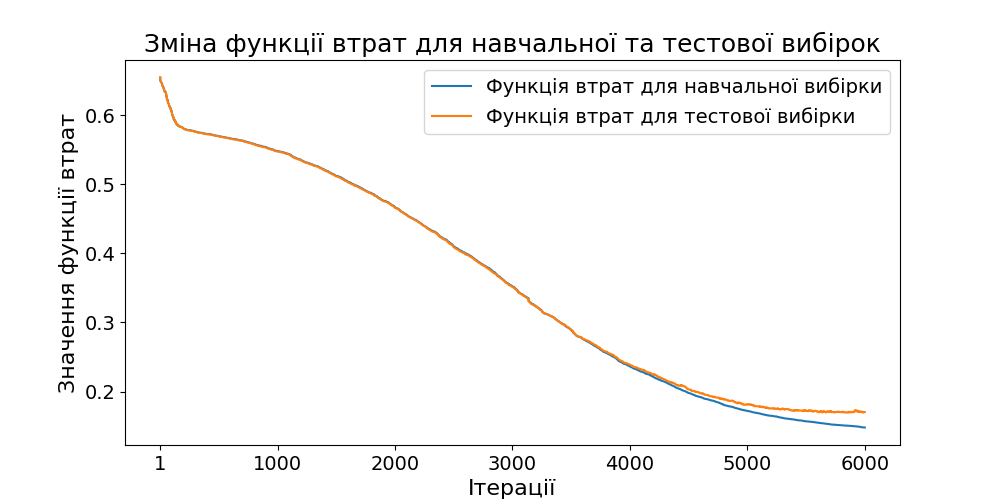
\includegraphics[width=\textwidth]{/home/loipoi/bachelor-diploma/pictures/binary_classification_image/mlp_with_spm_without_overfit.png}
		\caption{}
	\end{subfigure}	
	\begin{subfigure}[b]{0.32\textwidth}
		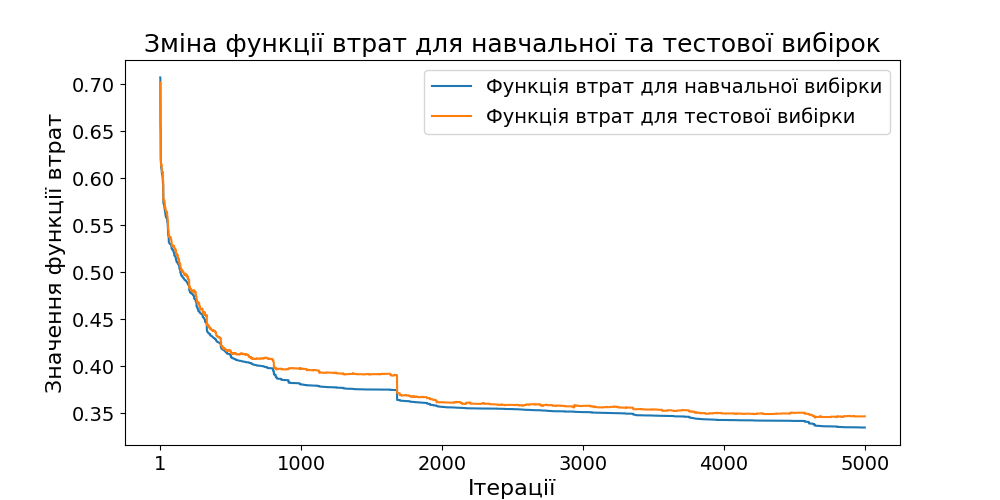
\includegraphics[width=\textwidth]{/home/loipoi/bachelor-diploma/pictures/binary_classification_image/ea_without_overfit.png}
		\caption{}
	\end{subfigure}
	
	\caption{Графіки залежності функцій втрат від кількості ітерацій для методів: (a) MLP with gradient descent, (б) MLP with single-point mutation, (в) $(1+\lambda)$-EA with GP encoding, для задачі бінарної класифікації зображень}
	\label{fig_losses_bc_id}
\end{figure}

З цих результатів можна бачити, що усі три моделі досягають приблизно однакових метрик. Найкращі результати моделі MLP with gradient descent, MLP with single-point mutation та $(1+\lambda)$-EA with GP encoding мали після 69, 5855 та 4645 епох відповідно, але якщо проаналізувати часову складову результатів, то видно, що модель MLP with gradient descent має доволі гарні результати, а саме найкращий показник функції втрат на тестовій вибірці до якого модель зійшлась за 1.7166 секунду, в той час, як моделі MLP with single-point mutation та $(1+\lambda)$-EA with GP encoding зійшлись до приблизно таких же показників за значно більший час, а саме 46.5702 та 3452.8294 секунд відповідно.

На графіках б та в рисунку \ref{fig_losses_bc_id} також можна помітити, що є певні плато в які моделі ненадовго потрапляли, таким чином це ще раз підтверджує необхідність модифікації цих алгоритмів, оскільки наразі вони мають цей недолік.

Розглянемо задачу багатокласової класифікації табличних даних. Як вже згадувалося, для цього ми використовували датасет Human Activity Recognition with Smartphones. Оптимальні гіперпараметри для усіх трьох моделей наведені у попередньому розділі. Моделі тренувалися протягом 100, 40000 та 15000 епох відповідно.

\begin{table}[ht]
	\centering
	\begin{adjustbox}{max width=\textwidth}
		\begin{tabular}{|c|c|c|c|}
			\hline 
			& MLP with gradient descent & MLP with single-point mutation & $(1+\lambda)$-EA with GP encoding \\
			\hline 
			Accuracy & 0.9389 & 0.9532 & 0.8992 \\
			\hline 
			Precision & 0.9409 & 0.9540 & 0.9024 \\
			\hline
			Recall & 0.9363 & 0.9520 & 0.8964 \\
			\hline
			F1-score & 0.9386 & 0.9530 & 0.8994 \\
			\hline
		\end{tabular}
	\end{adjustbox}
	\caption{Метрики на найкращій ітерації кожної моделі для задачі багатокласової класифікації табличних даних}
	\label{metrics_mc_td_results}
\end{table}

\begin{figure}[ht]
	\centering
	\begin{subfigure}[b]{0.32\textwidth}    
		\includegraphics[width=\textwidth]{/home/loipoi/bachelor-diploma/pictures/multiclass_classification_tabular/mlp_with_gd.png}
		\caption{}
	\end{subfigure}	
	\begin{subfigure}[b]{0.32\textwidth}
		\includegraphics[width=\textwidth]{/home/loipoi/bachelor-diploma/pictures/multiclass_classification_tabular/mlp_with_spm.png}
		\caption{}
	\end{subfigure}	
	\begin{subfigure}[b]{0.32\textwidth}
		\includegraphics[width=\textwidth]{/home/loipoi/bachelor-diploma/pictures/multiclass_classification_tabular/ea.png}
		\caption{}
	\end{subfigure}
	
	\caption{Графіки залежності функцій втрат від кількості ітерацій для методів: (a) MLP with gradient descent, (б) MLP with single-point mutation, (в) $(1+\lambda)$-EA with GP encoding, для задачі багатокласової класифікації табличних даних}
	\label{fig_losses_mc_td}
\end{figure}

Результати для моделі MLP with gradient descent показують, що після 100 епох вона досягла оптимальних значень метрик, за 5.6244 секунд. Для моделі MLP with single-point mutation оптимальні значення були досягнуті після 30355 епох за 301.4574 секунду. Модель $(1+\lambda)$-EA with GP encoding досягла найкращих результатів після 13151 епох за 98058.2898 секунди. Результуючі метрики на найкращій ітерації для усіх трьох моделей представлені в таблиці~\ref{metrics_mc_td_results}. Графіки зміни функцій втрат для кожної моделі представлені на рисунку~\ref{fig_losses_mc_td}.

З цих результатів можна бачити, що моделі MLP with gradient descent та MLP with single-point mutation показали трохи кращі результати за $(1+\lambda)$-EA with GP encoding, але метод $(1+\lambda)$-EA with GP encoding виділився легкістю контролювання, оскільки для покращення його метрик нам потрібно просто збільшити експресивність кодувань, а саме збільшити значення гіперпараметрів tree\_depth, або $\lambda$, в той час, щоб покращити значення метрик методів MLP with gradient descent та MLP with single-point mutation нам потрібно робити оптимізацію гіперпараметрів, у першому випадку нам потрібно буде підбирати параметри, які наведені у таблиці \ref{tab_hyperparameters_for_mlp_with_gd}, а для другого випадку потрібно буде підбирати значення гіперпараметрів з таблиці \ref{tab_hyperparameters_for_mlp_with_sp_mut}. Якщо проаналізувати часову складову результатів, то видно, що модель MLP with gradient descent має значно кращі результати, ніж два інші методи, в той час, як модель $(1+\lambda)$-EA with GP encoding має значно більший час тренування, а саме 98058.2898 секунди.

Перейдемо до останньої задачi для якої ми робили порiвняння моделей -- багатокласової класифiкацiї зображень з використанням датасету Chest X-Ray Images (Pneumonia). Зазначимо, що моделі тренувалися протягом 4, 4000 та 3000 епох відповідно. 

\begin{table}[ht]
	\centering
	\begin{adjustbox}{max width=\textwidth}
		\begin{tabular}{|c|c|c|c|}
			\hline 
			& MLP with gradient descent & MLP with single-point mutation & $(1+\lambda)$-EA with GP encoding \\
			\hline 
			Accuracy & 0.7420 & 0.7356 & 0.6955 \\
			\hline 
			Precision & 0.7705 & 0.7677 & 0.7195 \\
			\hline
			Recall & 0.7037 & 0.6936 & 0.6634 \\
			\hline
			F1-score & 0.7356 & 0.7288 & 0.6903 \\
			\hline
		\end{tabular}
	\end{adjustbox}
	\caption{Метрики на найкращій ітерації кожної моделі для задачі багатокласової класифікації зображень}
	\label{metrics_mc_id_results}
\end{table}

\begin{figure}[ht]
	\centering
	\begin{subfigure}[b]{0.32\textwidth}    
		\includegraphics[width=\textwidth]{/home/loipoi/bachelor-diploma/pictures/multiclass_classification_image/mlp_with_gd.png}
		\caption{}
	\end{subfigure}	
	\begin{subfigure}[b]{0.32\textwidth}
		\includegraphics[width=\textwidth]{/home/loipoi/bachelor-diploma/pictures/multiclass_classification_image/mlp_with_spm.png}
		\caption{}
	\end{subfigure}	
	\begin{subfigure}[b]{0.32\textwidth}
		\includegraphics[width=\textwidth]{/home/loipoi/bachelor-diploma/pictures/multiclass_classification_image/ea.png}
		\caption{}
	\end{subfigure}
	
	\caption{Графіки залежності функцій втрат від кількості ітерацій для методів: (a) MLP with gradient descent, (б) MLP with single-point mutation, (в) $(1+\lambda)$-EA with GP encoding, для задачі багатокласової класифікації зображень}
	\label{fig_losses_mc_id}
\end{figure}

Результати для моделі MLP with gradient descent показують, що після 4 епох вона досягла оптимальних значень метрик, за 0.1965 секунди. Для моделі MLP with single-point mutation оптимальні значення були досягнуті після 3198 епох за 19.0337 секунду. Модель $(1+\lambda)$-EA with GP encoding досягла найкращих результатів після 2382 епохи за 43179.4566 секунди. Результуючі метрики на найкращій ітерації для усіх трьох моделей представлені в таблиці~\ref{metrics_mc_id_results}. Графіки зміни функцій втрат для кожної моделі представлені на рисунку~\ref{fig_losses_mc_id}.

З цих результатів можна бачити, що усі три моделі досягають приблизно однакових метрик. Проаналізувавши часову складову результатів видно, що модель MLP with gradient descent має доволі гарні результати, а саме найкращий показник функції втрат на тестовій вибірці до якого модель зійшлась за 0.1965 секунд, в той час, як моделі MLP with single-point mutation та $(1+\lambda)$-EA with GP encoding зійшлись до приблизно таких же показників за значно більший час, а саме 19.0337 та 43179.4566 секунд відповідно.

Провівши експерименти для чотирьох різних задач можна зробити висновок, що усі три методи можуть досягти однаково високих показників, або порівнюваних, але в кожного з методів є свої сильні та слабкі сторони. 

Модель MLP with gradient descent має швидкий час збіжності до точки оптимуму в порівнянні з іншими двома методами, але при цьому таку модель важко контролювати. Оскільки, якщо модель демонструє погані метрики, то ми не можемо точно сказати, як це покращити, чи збільшувати, наприклад, параметр learning\_rate, чи ні, оскільки через його збільшення модель може перескочити оптимальну точку, а через зменшення, навпаки дуже довго збігатися до неї, тому для того, щоб отримати гарні результати, потрібно проводити оптимізацію гіперпараметрів. Але в той же час, як ми бачили на прикладі класифікації зображень, якщо функція втрат доволі гладка і якщо початкова ініціалізація ваг достатньо вдала, то метод на основі градієнтного спуску доволі швидко збігається до точки оптимуму, це відбувається тому, що в цьому методі оптимізація параметрів моделі (а саме ваг та bias) відбувається в усіх напрямках, тобто за одну ітерацію значення кожного з параметрів зміщується в оптимальну сторону, на відміну від методу MLP with single-point mutation, під час якого за одну ітерацію змінються значення тільки одних ваг, через це модель просто спускається до точки оптимуму одразу по усім осям. Таким чином, можна зробити висновок, що якщо для поточної задачі важлива швидкість навчання моделі, то MLP with gradient descent є гарним вибором, однак, якщо нам важливо мати контроль над моделлю, то краще обрати іншу модель.

Як видно з експериментів модель MLP with single-point mutation більш повільно збігається до точки оптимуму, ніж MLP with gradient descent, але в той же час не надто повільно. Але вона має перевагу в термінах контролювання, ця модель має значно менше гіперпараметрів для оптимізації, всього два: hidden\_layer\_sizes та scale\_for\_mutation. Хоча все одно важко сказати, як саме потрібно змінювати значення цих гіперпараметрів, якщо модель демонструє незадовільний результат, але за рахунок того, що гіперпараметрів значно менше, ніж у моделі MLP with gradient descent, зменшується простір пошуку гіперпараметрів, таким чином ми можемо за n кількість ітерацій пройти більше в глибину і підібрати кращі значення цих параметрів, ніж ми могли б це зробити з такою ж кількістю ітерацій, але для моделі MLP with gradient descent. Але як вже було зазначено, за одну ітерацію модель потенційно змінює тільки одне значення ваг, при чому це значення може виявитися гіршим, ніж те значення, яке було до цього, через що нове значення не прийметься, тобто за одну ітерацію значення взагалі в результаті може не змінитися, саме через це ця модель може значно довше збігатися до точки оптимуму.

Останньою розглянемо модель $(1+\lambda)$-EA with GP encoding. Як видно з експериментів, а саме з результатів для задач класифікації зображень та задачі багатокласової класифікації табличних даних, модель на цих даних демонструє дуже погані результати в термінах часу. Це відбувається з кількох причин: 

--- Для задач багатокласової класифікації проблема в тому, що цей алгоритм погано масштабується по відношенню до кількості класів, оскільки для того, щоб отримати передбачення ймовірностей для кількості класів більшу за 2, потрібно, щоб модель на виході давала відповідну кількість чисел, а для цього потрібно використовувати одне дерево на кожний клас. У такому випадку наш індивід складається з декількох дерев, які передбачають ймовірності належності вхідного прикладу до відповідних класів. Кожне з цих дерев повинно бути такої ж глибини, як і у випадку бінарної класифікації. В задачі бінарної класифікації одне дерево відповідає за передбачення ймовірності належності вхідного прикладу до класу 1. Це означає, що ми використовуємо ціле дерево для моделювання залежностей для передбачення одного класу. Під час тренування такого алгоритму ми використовували наступний підхід -- на кожній ітерації випадковим чином обирався вузол дерева і значення в ньому замінювалося на якесь інше випадково обране значення, тобто за одну ітерацію дерево вчиться робити кращі передбачення тіяк можна бачитильки для одного класу, що також значно сповільнює даний алгоритм. Також, чим більший розмір даних (кількість ознак або кількість прикладів), тим довше триває навчання. Це твердження стосується як алгоритмів MLP with gradient descent, так і MLP with single-point mutation. Але якщо для реалізації алгоритму MLP with gradient descent ми використовували популярну бібліотеку scikit-learn, яка покращувалася багато років ком'юніті та командою розробників, то для реалізації $(1+\lambda)$-EA with GP encoding ми скористалися бібліотекою Deap. Ця бібліотека є найпопулярнішою для реалізації генетичних алгоритмів. Однак, оскільки генетичні алгоритми в цілому менш популярні серед ком'юніті порівняно з нейронними мережами, до покращення цієї бібліотеки було докладено значно менше зусиль і часу. Тому під час виконання цього алгоритму частина часу витрачається через можливі неоптимальні рішення в цій бібліотеці.

--- Для задачі бінарної класифікації алгоритм досить повільно навчається через те, що деякі методи в бібліотеці, за допомогою якої ми реалізовували алгоритм $(1+\lambda)$-EA with GP encoding, гірше оптимізовані для випадку, коли на вході дається велика кількість даних (велика кількість ознак або спостережень).

Але незважаючи на те, що ця модель на великій кількості даних, або для задач багатокласової класифікації може навчатися велику кількість часу, ця модель має свої плюси. По перше, якщо набір даних невеликого розміру та задача -- бінарна класифікація, то як ми бачимо в таблиці \ref{metrics_bc_td_results} цей алгоритм може показувати такі ж гарні результати в плані метрик, як і MLP. 

По-друге, навіть якщо ми маємо великий обсяг даних або перед нами стоїть задача багатокласової класифікації, ми все одно можемо використовувати цей алгоритм. Це можливо, оскільки алгоритм легко контролювати. Якщо він показує погані результати при поточній конфігурації, нам точно відомо, як покращити результати. Для покращення результатів потрібно додати більше експресивності до кодувань. Це можна зробити, збільшивши глибину дерева, що дозволить алгоритму вивчати більш складні залежності в даних та моделювати більш глибокі функції. 

Або ж можна збільшити значення параметру $\lambda$, що призведе до генерації більшої кількості різноманітних нащадків на кожній ітерації. Це сприятиме більш глибокому пошуку по ознакам в даних. Також можна збільшити обидва параметри одночасно. Однак варто звернути увагу, що збільшення цих параметрів призведе до більшого часу тренування. Збільшення глибини дерева потребує обрахування більшої кількості функцій, а збільшення значення параметру $\lambda$ вимагає проганяння усіх даних через більшу кількість дерев. 

Додатково цей алгоритм має ще одну перевагу, а саме, якщо нам точно відомо, що в наших даних якісь ознаки мають залежність у вигляді певної функції, наприклад додавання, то ми можемо зафіксувати цю відому структуру в дереві і не змінювати її під час навчання, таким чином ми врахуємо цю залежність і вивчимо усі інші залежності між ознаками. 

Також до переваг цього алгоритму можна віднести його інтерпретованість для даних низької розмірності. Якщо дані мають невелику кількість ознак, ми можемо навчити цей алгоритм з задовільною швидкістю. Оскільки алгоритм моделює функціональну залежність між різними ознаками, ми отримаємо невелике дерево. Це тому, що для невеликої кількості ознак вистачить дерева з малою глибиною, щоб врахувати усі залежності між ознаками. Таке дерево буде доволі легко інтерпретувати. 

Підсумовуючи, даний алгоритм добре підходить для задач де важливо мати контрольованість над процесом навчання, для прикладу, в задачах де наперед відомо про певні залежності в даних, а саме в аналізі медичних даних, де ми можемо знати якісь патофізіологічні залежності, а також, якщо ми маємо дані малої розмірності і при цьому нам важливо бути спроможним інтерпретувати результат роботи алгоритму.

\chapconclude{\ref{chap:practice}}

У цьому розділі проведено експерименти для порівняння ефективності моделей MLP with gradient descent, MLP with single-point mutation та $(1+\lambda)$-EA with GP encoding для задач бінарної та багатокласової класифікації на різних наборах даних. Гіперпараметри налаштовувалися за допомогою байєсівської оптимізації. В ході експериментів було показано наступне.

Для задачі бінарної класифікації табличних даних усі моделі досягли однакових метрик, а саме f1-score для моделі MLP with gradient descent = 0.7966, для моделі MLP with single-point mutation = 0.7921, для моделі $(1+\lambda)$-EA with GP encoding = 0.8381. Але в термінах часу MLP with gradient descent та $(1+\lambda)$-EA with GP encoding показали значно кращі результати за MLP with single-point mutation. Модель MLP with gradient descent виявилася на 92.844\% швидше за MLP with single-point mutation, а модель $(1+\lambda)$-EA with GP encoding на 92.194\%. 

Для задачі бінарної класифікації зображень усі моделі показали співставні результати, а саме f1-score для моделі MLP with gradient descent = 0.9716, для моделі MLP with single-point mutation = 0.9687, для моделі $(1+\lambda)$-EA with GP encoding = 0.9526. Але в термінах часу значно виграє модель MLP with gradient descent, яка тренувалася на 96.314\% швидше за MLP with single-point mutation та на 99.950\% швидше за $(1+\lambda)$-EA with GP encoding.

Також варто зазначити, що для задач бінарної класифікації на графіках функцій втрат моделей MLP with single-point mutation та $(1+\lambda)$-EA with GP encoding видно, що при поточній реалізації моделі мають недолік, а саме вони в певні моменти виходять на плато. Таким чином для того, щоб це змінити варто додати прискорення, як тільки функція втрат довго не змінюється, або змінюється повільно.

Для задач багатокласової класифікації табличних даних та картинок також усі моделі досягли однакових результатів: для табличних даних f1-score моделі MLP with gradient descent = 0.9386, моделі MLP with single-point mutation = 0.9530, моделі $(1+\lambda)$-EA with GP encoding = 0.8994; для зображень f1-score моделі MLP with gradient descent = 0.7356, моделі MLP with single-point mutation = 0.7288, моделі $(1+\lambda)$-EA with GP encoding = 0.6903. Але знову видно, що в термінах часу MLP with gradient descent значно виграє. Він виявився на 98.134\% швидше за MLP with single-point mutation та на 99.994\% швидше за $(1+\lambda)$-EA with GP encoding для табличних даних та на 98.968\% швидше за MLP with single-point mutation та на 99.999\% швидше за $(1+\lambda)$-EA with GP encoding для зображень.

У підсумку можна сказати, що MLP with gradient descent працює швидше за інші моделі і при цьому має такі ж метрики, як і інші моделі, але з іншої сторони його важче контролювати та він є менш інтерпретованим. MLP with single-point mutation має кращу контрольованість, але повільніше збігається до точки оптимуму. $(1+\lambda)$-EA with GP encoding має найкращу контрольованісь та інтерпретованість, але значно повільніше навчається.